\section[Navegación]{Navegación}

\begin{frame}
  \Huge
  Navegación
\end{frame}

\begin{frame}\frametitle{Planeación de movimientos}
  El problema de la planeación de movimientos comprende cuatro tareas básicas:
  \begin{itemize}
  \item Navegación (encontrar una ruta por el espacio libre de un punto inicial a uno final). Si la ruta está parametrizada con repecto al tiempo, se dice que es una trayectoria.
  \item Mapeo (construir una representación del ambiente a partir de las lecturas de los sensores y la configuración)
  \item Localización (determinar la configuración a partir de un mapa y de lecturas de los sensores)
  \item Barrido (pasar un actuador por todos los puntos de un subespacio)
  \end{itemize}
  Comúnmente el mapeo y la localización se realizan al mismo tiempo en el proceso conocido como SLAM (\textit{Simultaneous Localization and Mapping})
\end{frame}

\begin{frame}\frametitle{Celdas de ocupación}
  Es una discretización del espacio con una resolución determinada donde a cada celda se le asigna un número $p\in[0,1]$ que indica su nivel de ocupación.
  \begin{itemize}
  \item En un enfoque probabilístico, $p$ indica la certeza de que la celda esté ocupada: 0, certeza de que está libre, 1, certeza de que está ocupada, 0.5, no se tiene información.
  \item En este curso, los niveles de ocupación solo serán 0 o 1.
 Para evitar el manejo de flotantes, el nivel de ocupación suele representarse con un entero en el intervalo [0,100] y un -1 si no hay información. 
  \end{itemize}
  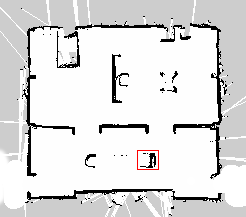
\includegraphics[width=0.4\textwidth]{Figures/OccupancyGrid.png}
  
\includegraphics[width=0.4\textwidth]{Figures/OccupancyGridZoom.png}
\end{frame}

\begin{frame}[containsverbatim]\frametitle{Ejercicio 1}
  Ejecute el comando:
  \begin{lstlisting}
    roslaunch bring_up path_planning.launch
  \end{lstlisting}
  Inspeccione el mapa en el visualizador RViz. Luego abra el archivo:
  \texttt{catkin\_ws/src/config\_files/maps/appartment.pgm}
  con cualquier editor de imágenes y modifíquelo.
  \\Detenga la ejecución y vuelva a correr el comando anterior. 
\end{frame}

\begin{frame}\frametitle{Planeación de rutas}
  Dado un espacio de configuraciones $Q$ con espacio libre $Q_{free}\subset Q$ y espacio ocupado $Q_{occ}\subset Q$, la planeación de rutas consiste en contrar un mapeo:
  \[f: [0,1] \rightarrow Q_{free} \qquad \textrm{con}\qquad f(0) = q_s\qquad f(1)=q_g\]
  donde $q_s$ y $q_g$ son las configuraciones inicial y meta, respectivamente. Es decir, se debe encontrar una secuencia de puntos del espacio libre que permitan al robot moverse del punto inicial al punto meta sin chocar. Los métodos para planear rutas se pueden agrupar en:
  \begin{itemize}
  \item Basados en búsqueda en grafos (A*, Dijkstra)
    \begin{itemize}
    \item En un mapa de celdas de ocupación, cada celda libre es un nodo del grafo.
    \item Cada nodo está conectado con las celdas vecinas del espacio libre. 
    \end{itemize}
  \item Basados en muestreo (RRT)
  \item Variacionales
  \end{itemize}
\end{frame}

\begin{frame}\frametitle{El algoritmo A*}
    \begin{algorithm}[H]
    \footnotesize
    \DontPrintSemicolon
    \KwData {Mapa $M$ de celdas de ocupación, configuración inicial $q_{start}$, configuración meta $q_{goal}$}
    \KwResult{Ruta $P=[q_{start},q_1, q_2, \dots , q_{goal}]$}
    \;
    Obtener los nodos $n_s$ y $n_g$ correspondientes a $q_{start}$ y $q_{goal}$\;
    Lista abierta $OL = \emptyset$ y lista cerrada $CL = \emptyset$\;
    \ForAll{Nodo $n \in M$}
    {
      $g(n) = \infty \qquad f(n) = \infty$\;
    }
    Agregar $n_s$ a $OL$\;
    $g(n_s) = 0 \qquad f(n_s) = 0$\;
    Nodo actual $n_c = n_s$\;
    \While{$OL\neq \emptyset$ y $n_c\neq n_g$}
    {
      Seleccionar de $OL$ el nodo $n_c$ con el menor valor $f$ y agregar $n_c$ a $CL$\;
      \ForAll{Vecino $n$ de $n_c$}
      {
        Calcular los valores $g$ y $h$ para el nodo $n$\;
        \If{$g < g(n)$}
        {
          $g(n) = g\qquad f(n) = g + h \qquad Previo(n) = n_c$
        }
      }
      Agregar a $OL$ los vecinos de $n_c$ que no estén ya en $OL$ ni en $CL$\;
    }
    \If{$n_c\neq n_g$}{Anunciar Falla}
    Obtener la configuración $q_i$ para cada nodo $n_i$ de la ruta\;
  \end{algorithm}
\end{frame}

\begin{frame}\frametitle{El algoritmo A*}
  El valor $g$ es una función de costo y el algoritmo A* siempre devolverá la ruta que minimice el costo total del nodo inicial al nodo meta. Las funciones más comunes son:
  \begin{itemize}
  \item Distancia de Manhattan: $d(p_1, p_2) = |p_{1_x} - p_{2_x}| + |p_{1_y} - p_{2_y}|$
  \item Distancia Euclidiana: $d(p_1, p_2) = \left( (p_{1_x} - p_{2_x})^2 + (p_{1_y} - p_{2_y})^2 \right)^{1/2}$
  \end{itemize}
  En la función $g$ se puede incluir cualquier criterio para planear una ruta: la más corta, la más rápida, la más segura, etc.\\
  La heurística $h$ sirve para expandir menos nodos y es una función que debe \textit{subestimar} el costo real de llegar de un nodo $n$ al nodo meta $n_g$. La distancia Euclidiana y la distancia de Manhattan son dos funciones también muy usadas como heurísticas. 
\end{frame}

\begin{frame}[containsverbatim]\frametitle{Ejercicio 2}
  Ejecute el comando:
  \begin{lstlisting}
    roslaunch bring_up path_planning.launch
  \end{lstlisting}
  En otra terminal, ejecute el comando:
  \begin{lstlisting}
    rosrun exercises a_star.py
  \end{lstlisting}
  Utilizando la GUI calcule una ruta desde la posición del robot hasta el punto (0,0). En el visualizador \texttt{RViz} se mostrará la ruta calculada.\\
  \begin{figure}
    \centering
    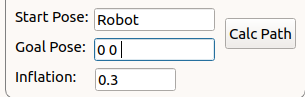
\includegraphics[width=0.35\textwidth]{Figures/Exercise1Gui.png}
    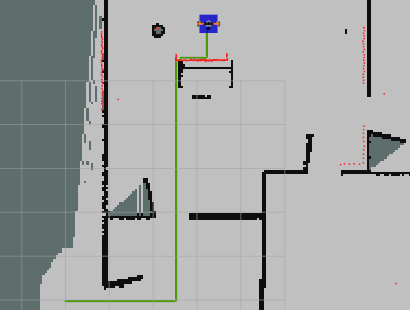
\includegraphics[width=0.35\textwidth]{Figures/Exercise1Rviz.png}
  \end{figure}
\end{frame}

\begin{frame}[containsverbatim]\frametitle{Ejercicio 2}
  Detenga la ejecución del programa \texttt{a\_star.py}. \\
    Modifique el archivo \texttt{catkin\_ws/src/exercises/scripts/a\_star.py} para utilizar distancia Euclidiana en lugar de distancia de Manhattan. Modifique las secciones marcadas con el comentario \texttt{\#Ejercicio}. 
    \lstinputlisting[language=Python,firstnumber=26]{Codes/AStar1.py}
    \lstinputlisting[language=Python,firstnumber=49]{Codes/AStar2.py}
    Ejecute nuevamente el comando
    \begin{lstlisting}
    rosrun exercises a_star.py
    \end{lstlisting}
    Y compare los resultados. 
\end{frame}

\begin{frame}\frametitle{Inflado de mapas}
  Para evitar que se calculen rutas por espacios por donde el robot en realidad no puede pasar debido a sus dimensiones, los obstáculos del mapa se deben \textit{inflar} cuando menos un número de celdas igual al radio del robot.\\
  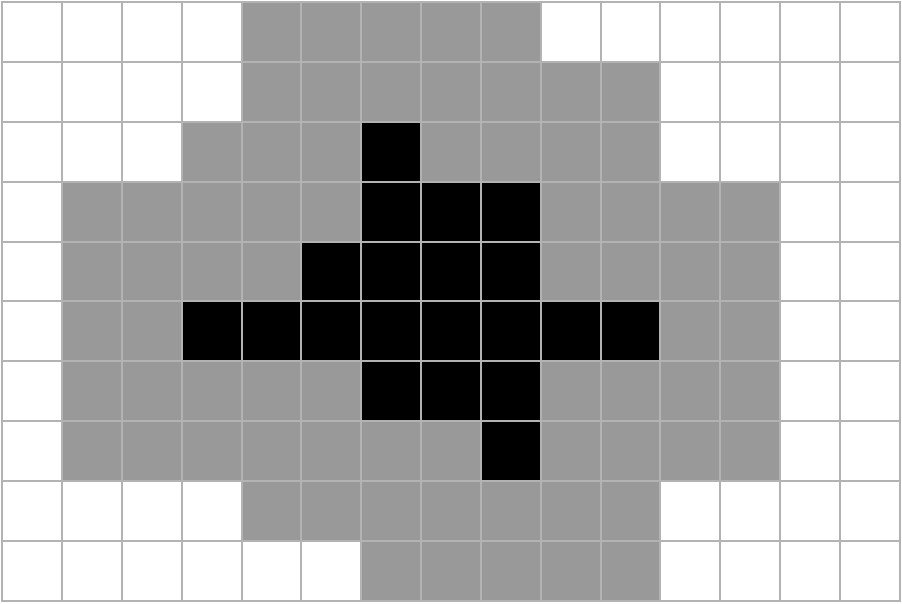
\includegraphics[width=0.45\textwidth]{Figures/Inflation.pdf}
  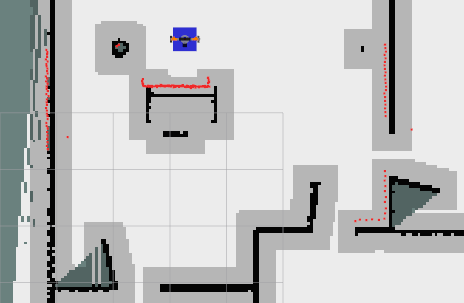
\includegraphics[width=0.45\textwidth]{Figures/Inflation.png}
\end{frame}

\begin{frame}[containsverbatim]\frametitle{Ejercicio 3}
  Modifique el archivo \texttt{catkin\_ws/src/exercises/scripts/inflation.py} para implementar el algoritmo de inflado de obstáculos:
  \lstinputlisting[language=Python,firstnumber=19]{Codes/Inflation.py}
  Ejecute el comando:
  \begin{lstlisting}
    roslaunch bring_up path_planning.launch
  \end{lstlisting}
  En otra terminal, ejecute el comando:
  \begin{lstlisting}
    rosrun exercises a_star.py
  \end{lstlisting}
  Y en una tercera terminal ejecute el comando
  \begin{lstlisting}
    rosrun exercises inflation.py
  \end{lstlisting}
\end{frame}

\begin{frame}\frametitle{Control de posición}
  Suponiendo que el robot está en la posición y orientación $(x,y, \theta)$ y que se quiere alcanzar la posición deseada $(x_g, y_g)$, como se muestra en la figura. Las leyes de control
  \begin{multicols}{2}
    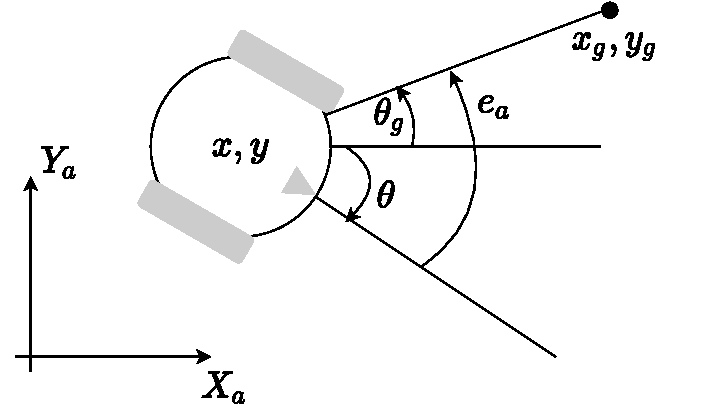
\includegraphics[width=0.5\textwidth]{Figures/GoalPose.pdf}
    \[\]
  \begin{eqnarray*}
    v &=& v_{max} e^{-e_a^2/\alpha}\\
    \omega &=& \omega_{max}\left(\frac{2}{1 + e^{-e_a/\beta}} - 1\right)
  \end{eqnarray*}
  \end{multicols}
  con $e_a = \textrm{atan2}(y_g - y, x_g - x) - \theta$, permiten que el robot alcance la posición deseada. Los parámetros $v_{max}$ y $\omega_{max}$ se deben seleccionar de acuerdo con las capacidades del robot. Las constantes $\alpha$ y $\beta$ permiten controlar qué tan rápido cambian la velocidad lineal y angular del robot. 
\end{frame}


\begin{frame}\frametitle{Seguimiento de rutas}
  El control de posición se puede utilizar para seguir una ruta si se fija como punto meta cada punto de la ruta, hasta alcanzar el último.
  \begin{figure}
    \centering
    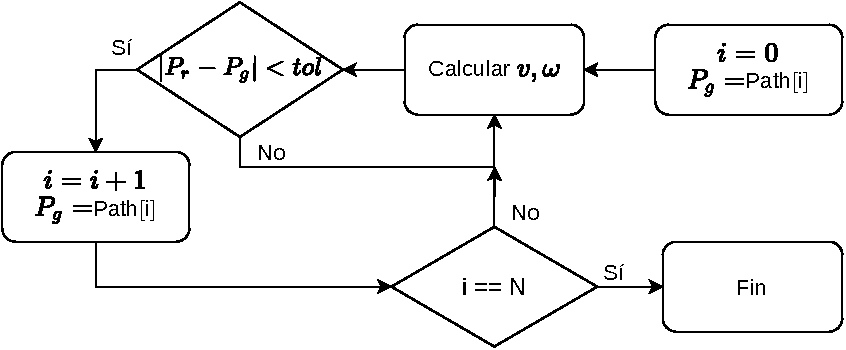
\includegraphics[width=0.6\textwidth]{Figures/PathFollowing.pdf}
  \end{figure}
\end{frame}


\begin{frame}[containsverbatim]\frametitle{Ejercicio 4}
  Ejecute el comando:
  \begin{lstlisting}
    roslaunch bring_up path_planning.launch
  \end{lstlisting}
  En otra terminal, ejecute el comando:
  \begin{lstlisting}
    roslaunch bring_up exercises_path_planning.launch
  \end{lstlisting}
  Utilizando RViz, envíe el robot a un punto meta:
  \begin{figure}
    \centering
    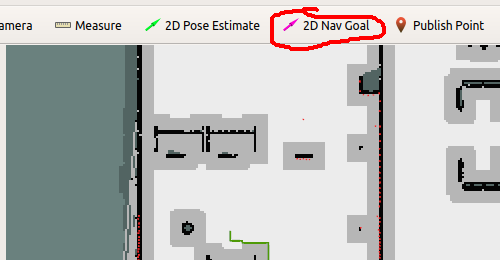
\includegraphics[width=0.5\textwidth]{Figures/Exercise4Rviz.png}
  \end{figure}
\end{frame}

\begin{frame}[containsverbatim]\frametitle{Ejercicio 4}
  Detenga la ejecución de los ejercicios. Abra el archivo \texttt{catkin\_ws/src/exercises/scripts/control.py} y modifique las constantes $v_{max}$, $\omega_{max}$, $\alpha$ y $\beta$.
  \lstinputlisting[language=Python,firstnumber=23]{Codes/Control.py}
  Vuelva a ejecutar el comando
  \begin{lstlisting}
    roslaunch bring_up exercises_path_planning.launch
  \end{lstlisting}
  Y compare el comportamiento del robot.
\end{frame}
